\documentclass{article}
\usepackage[utf8]{inputenc}
\usepackage{amsmath,amssymb,bm}
\usepackage{mathtools}
\usepackage{graphicx,caption}
\usepackage{listings}
\usepackage[margin=1.2in]{geometry}

\usepackage{titling}
\usepackage{lipsum}

\usepackage{parskip}

\usepackage{url}

\usepackage[
    style=authoryear-icomp,
    maxbibnames=9,
    maxcitenames=2,
    backend=biber
]{biblatex}
\addbibresource{sample.bib}

\setlength{\jot}{10pt}

\allowdisplaybreaks[1]

% Expectation symbol
\DeclareMathOperator*{\E}{\mathbb{E}}

% Math functions
\DeclareMathOperator{\Span}{span}

% Conditional
\newcommand\given[1][]{\:#1\vert\:}

% argmax
\DeclareMathOperator*{\argmax}{arg\,max}
\DeclareMathOperator*{\softmax}{soft\,max}

\graphicspath{{images/}}

\title{%
    Adversarial Text Generation\\
    \large NLP and Deep Learning --- Final Project
}

\author{%
    Andreas Holck Høeg-Petersen\\
    \texttt{anhh@itu.dk}
    \and
    Mathias Bastholm\\
    \texttt{mbas@itu.dk}
}

\begin{document}
\maketitle

\section{Introduction}\label{sec:introduction}

In recent years, Generative Adversarial Networks (GANs) have gained a lot of
traction in the Deep Learning community because of their impressive results in
image generation. The general idea is that a generator and a discriminator are
jointly trained to produce an image output that is seemingly indistinguishable
from non-generated images. This model were first described
in~\cite{Goodfellow2014GenerativeAN}.

We want to attempt to apply this strategy for text generation. The main
difficulty for this task is that whereas image outputs can be considered a
continuous value, a sentence is inherently discrete as it is a sequence of words
each of which is chosen by the model using the non-differentiable $argmax$
function. To remedy this, we propose a model where the discriminator is trained
to distinguish between the continuous outputs of a pre-trained encoder given a
`true' sentence from the generated, `fake' output stemming from our generator.

\begin{figure}[h]
    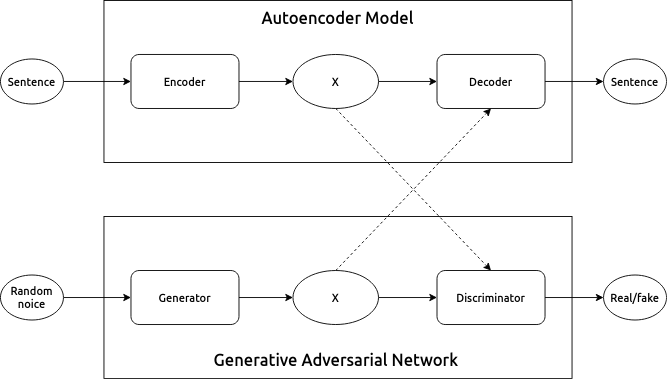
\includegraphics[width=\textwidth]{projectModel.png}
    \caption{% 
        Overview of the model architecture. The dotted lines from the
        $\mathbf{X}$s represents that the encoded and generated $\mathbf{X}$s
        will be fed to the discriminator and the decoder during training and
        evaluation, respectively.
    }\label{fig:projectModel}
\end{figure}

In our project, we will construct and train an autoencoder model that can encode
and decode a sentence from English to English. The encoded sentences are then
used as labelled training data for the discriminator, representing `true'
values. The job of the generator is to produce similar encodings but doing this
from random noise in a way that makes the discriminator unable to distinguish
between the encodings stemming from the autoencoder and the encodings stemming
from the generator.

Ideally, this would train the generator to produce sentence encodings that can
be fed to the decoder of the Transformer model which would then produce
meaningful sentences from this artificially generated input. See
Figure~\ref{fig:projectModel} for an overview of the complete model.

This project thus have two objectives: one is to construct a working autoencoder
that can map an English sentence to some hidden state $\mathbf{X}$ with a
corresponding decoder that can extract the original sentence from $\mathbf{X}$.
For convenience, we will refer to the encoder part of this model as the
`Teacher'. The second objective is to build a GAN network, where a generator ---
the `Student' --- must learn to produce approximations of $\mathbf{X}$.

The second objective is highly experimental as explained in
Section~\ref{sec:background}, where we will also describe other approaches at
using the GAN architecture for NLP problems. In Section~\ref{sec:method} we will
describe how we have build the different parts of the model and how we utilize
our dataset. Then in Section~\ref{sec:analysis} we will present our results and
discuss the shortcomings of the model\(s\), and in
Section~\ref{sec:furtherResearch} we will proceed to suggest improvements and
ideas for further research. Lastly, in Section~\ref{sec:conclusion} we conclude
on our project.


\section{Background}\label{sec:background}

Applications GANs have mainly focused on image generation and has not yet seen a
major breakthrough in text generation. As mentioned in
Section~\ref{sec:introduction}, this is because the discrete nature of text,
which is basically a sequence of words, requires a non-differentiable $argmax$
function to transform a probability distribution over a vocabulary to a single
value (ie.\ the word with the highest probability). This is depicted in
Figure~\ref{fig:argmaxGAN}.

\begin{figure}[h]
    \centering
    \captionsetup{width=0.8\textwidth}
    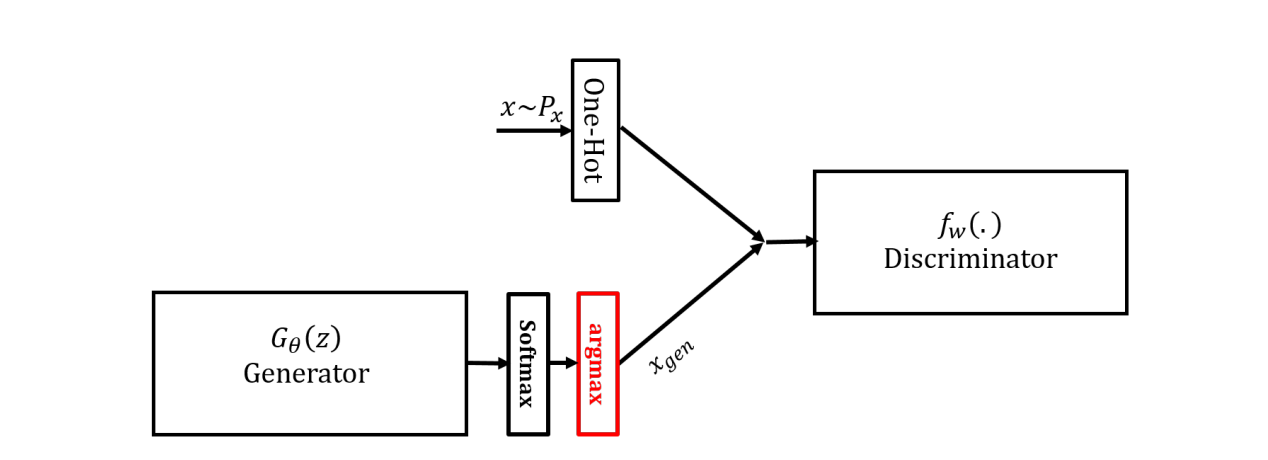
\includegraphics[width=0.8\textwidth]{argmaxGAN.png}
    \caption{%
        A simple GAN model where the generator output is run through an
        $argmax$ function before being given to the discriminator. This prevents
        gradients to flow from the discriminator to the generator.
        Source:~\cite{haidar2019textkdgan}.
    }\label{fig:argmaxGAN}
\end{figure}

There have been, however, multiple attempts at working around this issue.
According to~\cite{Chintapalli2019} these approaches can broadly be categorized
into three types:

\begin{itemize}
    \item Reinforcement Learning-based solutions
    \item The Gumbel-Softmax approximations
    \item Avoiding discrete spaces by working with the continuous output of the
        generaor
\end{itemize}

In this project, we follow the third approach, but in this section we will give
short introductions to the idea behind the two first.

As an example of an RL-based solution,~\cite{yu2016seqgan} proposes the SeqGAN
model, in which the generator is considered an RL-agent with states
$\mathbf{s}_t$ being the text generated at timestep $t$ and actions $\mathbf{a}$
being all the possible words to choose next. The agent then chooses its next
word (takes an action $a$) based on some policy function $\bm{\pi}(a \given
\bm{s}_t, \bm{\theta})$, where $\bm{\theta}$ are the parameters to be
optimized. Using Monte-Carlo rollouts to produce a number of different
sentences sharing a prefix $\bm{s}_t$, the discriminator then rewards each
sentence and the averaged reward is then used to perform gradient ascent on
$\bm{J}(\bm{\theta})$, where $\bm{J}$ is the performance measure of
$\bm{\theta}$. This approach alleviates some of the problems of training a GAN
for text generation, but it suffers from an unstable and slow training process,
convergence to sub-optimal local minima and and extremely large state-space.\

Another approach is to use the Gumbel-Softmax distribution to approximate a
one-hot encoding of a probability distribution passed through the $argmax$
function. This is the approach taken by~\cite{kusner2016gans}. Here, a
$d$-dimensional one-hot encoding vector $\bm{y}$ is approximated using

\begin{equation}
    \bm{y} = \softmax(\frac{1}{\tau}(\bm{h}+\bm{g}))
\end{equation}

where $\bm{h}$ is some hidden state (ie.\ of an RNN), $\bm{g}$ is drawn from a
Gumbel distribution and $\tau$ is a temperature parameter. This works because it
is differentiable and as $\tau \to 0$ the distribution of $\bm{y}$ will match
that we get from

\begin{equation}
    \bm{y} = \text{one\_hot}(\argmax_{i}(h_i + g_i))
\end{equation}

which again can be shown to be the same as sample $\bm{y}$ from a probability
distribution $\bm{p} = softmax(\bm{h})$ where $p_i = p(y_i=1), i = 1\dots d$.

Finally, for other examples on the third approach,
see~\cite{donahue2018adversarial} and~\cite{haidar2019textkdgan}.


\section{Method}\label{sec:method}

For all our models (autoencoders and GANs), we drew inspiration PyTorch
tutorials
(\cite{pytorchTutorialAtt},~\cite{pytorchTutorialTransformer},~\cite{pytorchTutorialGAN}),
tweaking them to our specific needs. The whole process (project development,
research, data collection, coding, training, experimentation and analysis) was
conducted during a 10-day period.

This section will describe this process, focusing on the final outcomes rather
than including all our intermediate steps and missteps.

\subsection{Dataset}\label{sec:dataset}

For training of the autoencoders, we simply needed dataset consisting of a large
number of English sentences. We obtained this from Universal Dependencies, where
used the `Universal Dependencies --- English Dependency Treebank Universal
Dependencies English Web Treebank v2.6 --- 2020--05--15' (\cite{silveira14gold})
consisting of 12,543 training sentences, 2,077 test sentences, 2,002 dev
sentences and a vocabulary of 16,654 training tokens. The data is annotated with
metadata such as lemmas and word classes, but we discarded this information as
it was not relevant for our purpose.

Furthermore, we also utilized another dataset intended for training
English-to-French translation. This dataset originates from
\url{https://tatoeba.org/eng/} and consists of 135,842 sentence pairs. We
discarded the French sentences and removed all duplicate sentences and sentences
of length smaller than 3, as well as splitting all sentences that contained
punctuations, questionmarks, exclamation points, etc. This gave us a set of
92,343 sentences, which we split 80/20 between training and testing/development,
and a vocabulary of 13,731 tokens.


\subsection{Models}\label{sec:models}

We developed two different versions of the autoencoder model and one GAN model.
These will be described in this subsection.

\subsubsection{The TransformerModel}\label{sec:transformermodel}

Our first autoencoder was based on~\cite{pytorchTutorialTransformer}. This model
consists of a very simple decoder, that is simply a feed-forward neural net that
takes a 2-dimensional tensor $X \in \mathbb{R}^{n \times k}$ and maps each of
the $n$ $k$-dimensional vectors of the sequence to a probability distribution
over the entire vocabulary which it then can convert to an output sequence using
$argmax$.

The encoder, however, is responsible for generating $X$ and it does so by using
the Transformer architecture as suggested in~\cite{vaswani2017attention} and
implemented in the PyTorch module \texttt{nn.Transformer}. For our purpose,
however, we only used the submodule \texttt{nn.TransformerEncoder}, which
consists of a stack of encoder layers that uses self-attention to focus on
specific, relevant parts of the input sequence in one go, and then passes its
output on to the next layer through a feed-forward network. As a preprocessing
step, before the input sequence is passed through the transformer, positional
encoding is added, as suggested in the paper (\cite{vaswani2017attention}).

This model also uses an embedding as its first layer. For embeddings, we use
pretrained word vectors from the \texttt{polyglot} Python package. These have an
embedding size of 64, which therefore what we use across all models. Note that
the next, RNN-based autoencoder uses the same embedding setup.


\subsubsection{RNN and Attention based Autoencoder}\label{sec:attnRNN}

In our second model, the heavy-lifting is switched from the encoder to the
decoder. Again, we utilize the attention mechanism, but this time it is combined
with an RNN architecture, more precisely a Gated Recurrent Unit (GRU). In this
model, the encoder is simply a GRU layer that processes the entire sequence and
then its final hidden state aswell as the output for each word in the sequence
is passed to the decoder.

The decoder has a bit more to it. On each timestep it takes in its own last
output (starting with the special \texttt{start-of-sequence}-token), a hidden
state (starting with the last hidden state of the encoder) and all the encoder
outputs. It then uses a linear layer (ie.\ a simple feed-forward network) to
calculate the attention weights by combining the input and the current hidden
state. The attention weights and the encoder outputs are then mulitplied
together using matrix multiplication and the result of this operation can then be
merged with the original input and passed through another linear layer to
produce a vector of size \texttt{(sequence\_length * hidden\_size)}.

In this vector, the decoder has now embedded all the information about where to
focus its attention, and it can pass this to a GRU just as in the encoder ---
however, opposite to the GRU in the encoder, the output of the recurrent layer
in the decoder is responsible for mapping back to actual words. This mapping is
finalized by an output linear layer that expands the hidden size to the size of
the vocabulary and then, finally, a $softmax$ operation converts the output to
probability distributions.

When the decoder outputs the special \texttt{end-of-sequence}-token it is
finished and the process terminates. Our implementation of this model is based
on~\cite{pytorchTutorialAtt}.


\subsubsection{GAN}\label{sec:modelGAN}

Our GAN model is modelled after our TransformerModel in an attempt to mimic the
inner mechanics of the network it is trying to imitate. As stated, a GAN
consists of a generator and a discriminator. The generator gets a vector of
random noise as input. This vector has dimensions \texttt{(max\_sequence\_length
* embedding\_size)}. The reason we set a parameter
\texttt{max\_sequence\_length} is because neural networks expects static sizes,
but since sentences can have different lengths, we set an upper bound. The
generator should, however, be able to encode its output in a way, that produces
sentences of length 0 to \texttt{max\_sequence\_length} (ie.\ by encoding an
\texttt{end-of-sequence}-token at some position).

The generator passes its input through a linear layer and then, as the
TransformerModel, adds positional encoding before it runs it through an encoder
stack (\texttt{nn.TransformerEncoder}). The final output has the same shape as
the output of the encoder part of the TransformerModel.

The discriminator has almost the same structure as the generator (it uses
positional encoding and an encoder stack), but the input differs and it outputs
a single number between 0 and 1. Recall, that the job of the discriminator is to
decide wether its input was generated from random noise via the generator or if
it was an encoding stemming from a real sentence passed through a trained
encoder. Thus, it is effectively a binary classifier, and its output should
describe its conviction that the input is `true'.

\subsection{Training}\label{sec:training}

Our training had to aspects: first, we had to train our autoencoders on
English-to-English sentence pairs, and then we had to train our GAN model. This
section will describe both.

\subsubsection{Training the autoencoders}

This part is pretty straight forward. We give the model a batch of sentences
which it then encodes and decodes again. Since the input sentence is also the
target sentence, the loss is simply the difference between the input and the
output. To calculate this loss, we use PyTorchs `nn.CrossEntropyLoss' which
takes the raw output of the model (ie.\ before it has been converted to a
probability distribution) and a target vector and then calculates the negative
log-likelihood loss. We use Stochastic Gradient Descent to update the weights of
the models.

There were some notable differences between the way we trained the
TransformerModel and the RNN-based model. For the TransformerModel we had good
results with a learning rate of 0.05, and we performed training on the entire
training set in batches of 8 and over the course of 25 epochs. We also trained
it another time with just 10 epochs, but this time without ignoring the padding
in the batches (when batching the data, not all sentences have the same length
and the smaller sentences are padded with the special \texttt{<PAD>}-token).
This makes the model achieve a lower loss much faster, as it quickly learns the
pattern of the padding tokens, but this often comes at the expense of the model
learning the actual sentence, which generally is what is of interest. However,
we wanted our Student model to learn both from a Teacher that had learned
padding and one that hadn't, so trained the autoencoders (Teacher) on both.

In training the RNN-based model we took inspiration
from~\cite{pytorchTutorialAtt}. This means we set the learning rate to 0.01 and
instead of training on the entire training set over multiple epochs, we let the
model randomly pick a data batch, train on that and then pick a new for 60,000
iterations. Furthermore, we used teacher forcing, where instead of letting the
output of the decoder be its own next input, we give the actual next input (from
the target sentence). This approach can lead to some terrible cases of
overfitting and preventing the model form learning its mistakes properly, but in
the right dose it can also help the model converge faster. Therefore, for each
training instance, we chose with 50\% probability wether to use teacher forcing
or not.


\subsubsection{Training the GAN model}

The training of the GAN model is the interesting and difficult process. Here, we
have to simultaneously train to different models that works towards opposite
goals. One, the generator, will have to learn how to maximise the probability
that the discriminator classifies its output as `true', while the other, the
discriminator, will have to learn to maximise the probability that it classifies
the output of the generator as `fake' while also classifying the output of the
Teacher (encoder) as `true'. So the two components engage in a mini-max game
with one another.

Formally, let $G$ and $D$ be the generator and the discriminator respectively
and let $x$ be the data representing a sentence (encoded or generated). Then,
$D(x)$ is the output of the discriminator given some data, and we want this to
be high when $x$ is `true' (stemming from the Teacher) and low when $x$ is
`fake' (generated by the Student). Let $z$ be some random noise, and then we
have that $G(z)$ is the output generated by the Student given some random noise.
So, the discriminator now tries to \textit{maximize} the probability that it
correctly classifies `true' and `fake' data, $\log D(x)$, and the generator
tries to \textit{minimize} the probability that the discriminator classifies its
outputs as `fake', $\log(1 - D(G(z)))$. As described in the original GAN
paper~\cite{Goodfellow2014GenerativeAN}, this can be formalised as:

\[
    \min_G \max_D V(D,G) = {\E}_{x \sim p_{data}(x)}\left[\log D(x)\right] +
        {\E}_{z \sim p_{z}(x)}\left[\log(1 - D(G(z)))\right]
\] 

where $p_{data}$ is the `true' distribution over the real data which the
generator tries to estimate, and $p_z$ is the estimated distribution that the
generator draws its samples from.

The way we do this is by following the approach suggested
by~\cite{Goodfellow2014GenerativeAN} and PyTorch GAN tutorial for image
generation~\cite{pytorchTutorialGAN}. This involves first giving the
discriminator a batch of `real' input (ie.\ input generated by the Teacher) and
then calculating the loss and the gradients based on its performance. Then we
give it a batch of `fake' data generated by the Student, again calculating the
loss and gradients. Then, before we move on to training the generator, we
perform our optimization step for the discriminator. When we then pass the
output of the generator through the discriminator, the discriminator has been
updated and the generator will have to learn to adjust to this. 

However, one could imagine that the generator could learn to just output random
words very well and that the discriminator would not be able to distinguish this
from a `real' sentence. Therefore, before training the generator, we also give
the discriminator a batch of `fake' data that has been generated by the encoder,
but when the encoder have gotten random words as input. This, in theory, should
force the generator to produce meaningful sentences (not just random words) for
it to be classified as `true' by the discriminator. This, by the way, is our own
adjustment to the training procedure.

It is worth noting, that training a GAN is known to be highly non-trivial
(\cite{Hui2018}) and even small variations in the hyperparameters, number of training
iterations or internal structure of the generator and/or discriminator can make
the model collapse spectacularly.

\section{Analysis}\label{sec:analysis}

In this section, we will present and discuss our results as well as give
suggestions for further improvements and research.

\subsection{Results}\label{sec:results}

Here are some plots:

\begin{figure}[h]
    \centering
    \begin{minipage}{0.45\textwidth}
        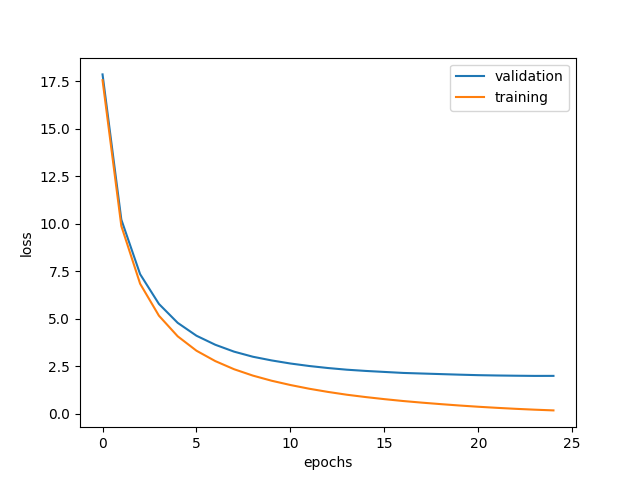
\includegraphics[width=0.9\textwidth]{transformer.png}
        \caption{%
            Transformer.png
        }\label{fig:transformer}
    \end{minipage}
    \begin{minipage}{0.45\textwidth}
        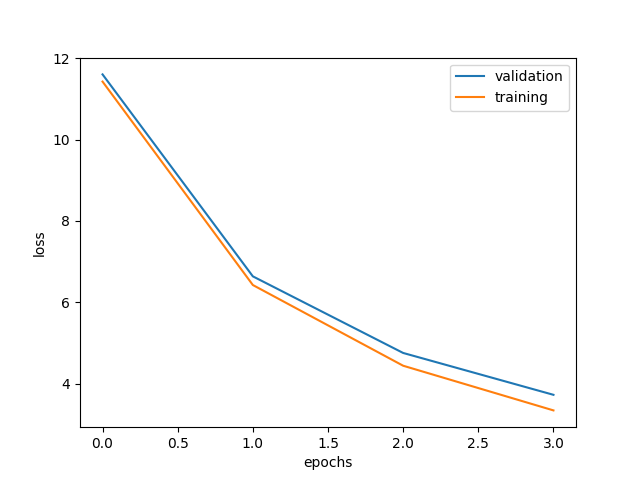
\includegraphics[width=0.9\textwidth]{transformer_padding-eos.png}
        \caption{%
            Transformer with padding and EOS
        }\label{fig:transformerPaddingEOS}
    \end{minipage}


\end{figure}


This is output from a TransformerModel during training:

\begin{verbatim}
| end of epoch   5 | time: 466.09s | valid loss  3.07 | valid ppl    21.58 | train loss  2.63
IN:  rwandan rebels are pushing their offensive south as fighting continues in the capital kigali . <EOS>
OUT: honest guys are noticed their interesting south as fighting awake in 
\end{verbatim}

\subsection{Discussion}\label{sec:discussion}

\textbf{These are notes:}

The GAN network is actually able to learn.
Sentences differ from random input.
Increasing the batch size of $z$ might help the generator.
The training breaks too soon
Discriminator gets to critical

`double\_batch' means that the generator is given a double sized batch for
training.

When we train the discriminator on encoded random words, $D(x)$ should be 0.5
for a perfect $D$ (because half of $x$ is `true' and the other half is `fake').
When omitting the encoded random words, $D(x)$ should be 1. Of course, for a
perfect network with a perfect $D$ and a perfect $G$, both $D(x)$ and $D(G(z))$
should be 0.5 

Training without encoded random words seem to make the generator take longer to
learn what to do with padding and EOS.\ However, it also seems to make the
network more stable.

The two output sentences in some of the GAN-training-output files are first the
output of $G$ given the fixed noise and then the output given random noise. Not
how they become almost identical.

SGD seem to make the network more stable, but it also tends to end up with small
sentences of identical words and a LOT of padding.

Training with no encoded random words went fine for very long, with the
generator actually being consistently better than the discriminator --- untill it
the hit a giant collapse (see
\texttt{../examples/GAN-training-output-double\_batch-Adam-no\_random.txt}
and~\ref{fig:doubleBatchAdamNoRandom} for evidence)

\begin{figure}[h]
    \captionsetup{width=\textwidth}
    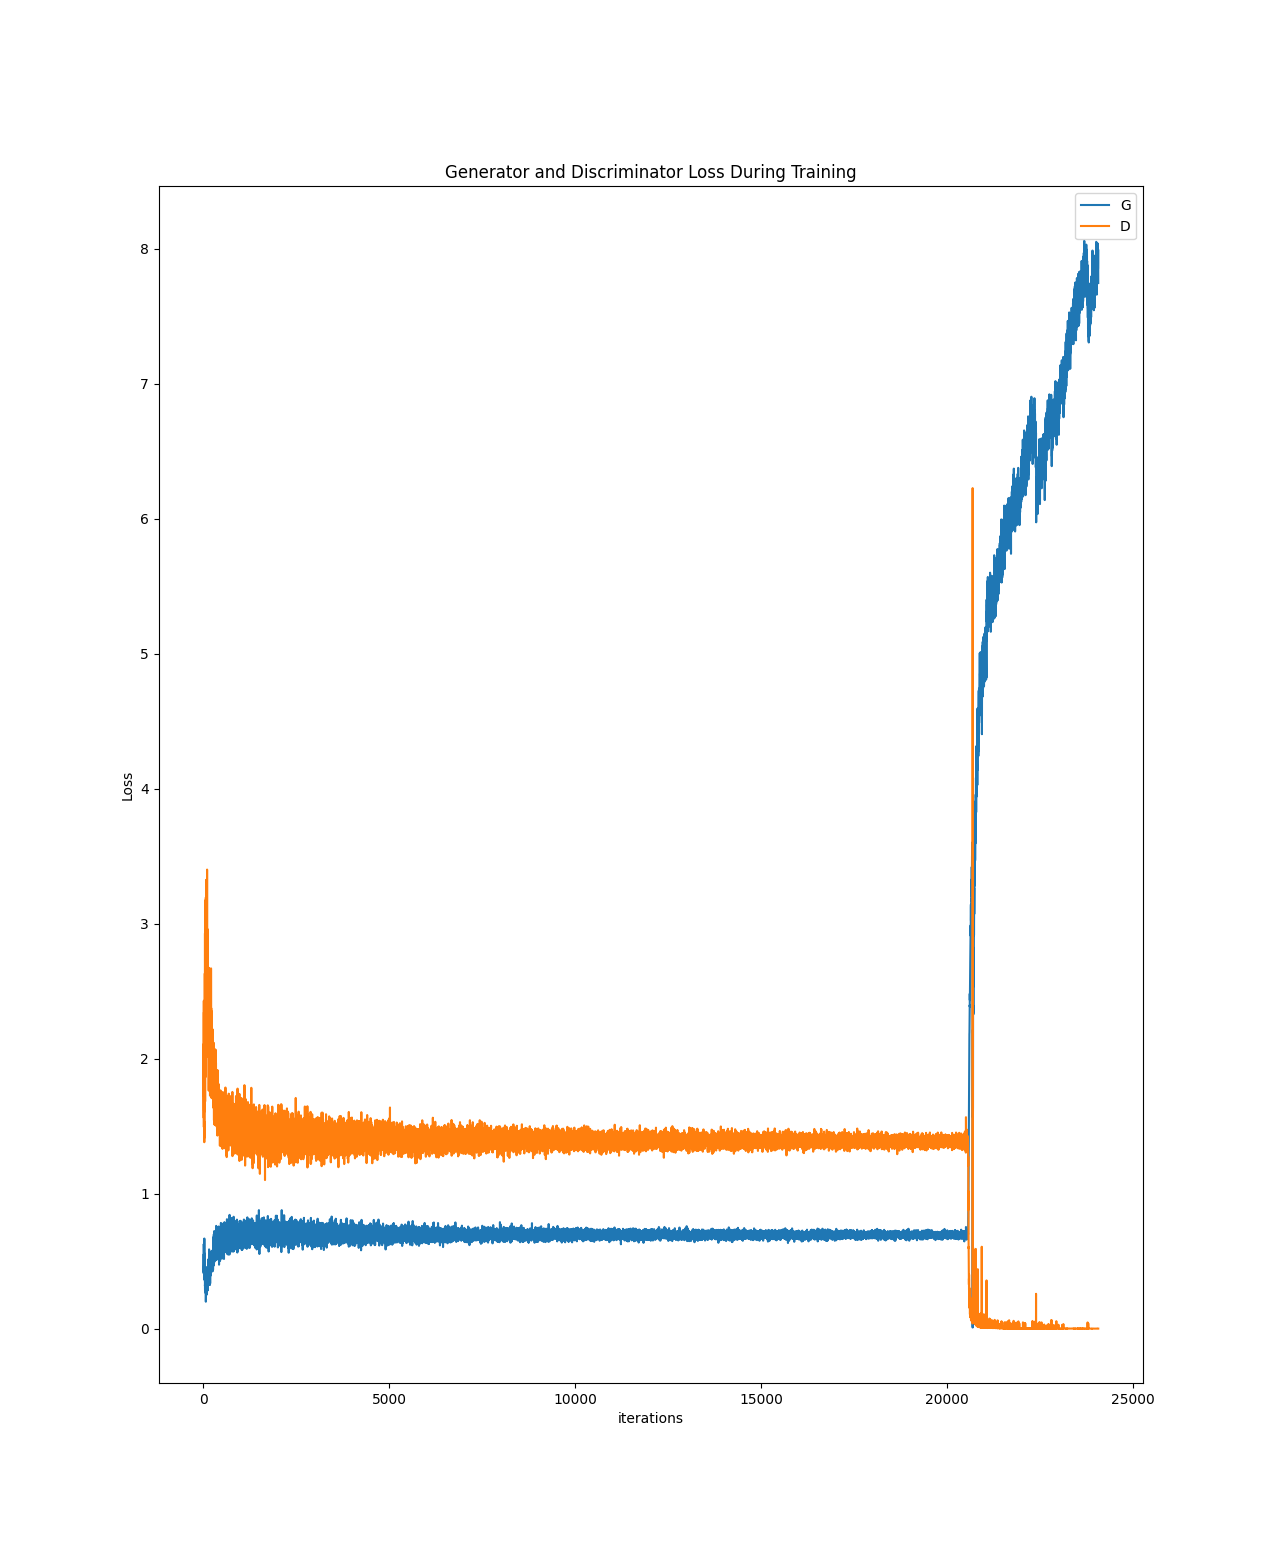
\includegraphics[width=\textwidth,height=12cm]{GAN-loss-double_batch-Adam-no_random.png}
    \caption{%
        GAN loss for setup with Adam, double batch and no encoded random words.
    }\label{fig:doubleBatchAdamNoRandom}
\end{figure}

\section{Further research}\label{sec:furtherResearch}


\section{Conclusion}\label{sec:conclusion}


\newpage
\printbibliography%

\end{document}

